\documentclass{beamer}

\usepackage[latin1]{inputenc}
\usepackage[T1]{fontenc}
\usepackage[frenchb]{babel}
\usepackage{lmodern}
\usepackage{graphicx}
\usepackage{multimedia}

\usetheme{Darmstadt}
\usecolortheme{seagull}

\logo{
\includegraphics[height=10mm]{ur1.png}}

\title{Soutenance de TIPE}
\subtitle{Comment la reconnaissance faciale du conducteur peut-elle am\'eliorer sa s�curit\'e au volant ?}
\author{S\'ebastien Blin, Pierre-Henri Collin, Amaury Louarn}
\institute{Universit\'e de Rennes 1}
\date{8 Avril 2014}

\AtBeginSection[]
{
  \begin{frame}
  \frametitle{Sommaire}
  \tableofcontents[currentsection, hideallsubsections]
  \end{frame} 
}

\begin{document}
	\begin{frame}
		\titlepage
	\end{frame}
	\begin{frame}
		\frametitle{Plan}
		\tableofcontents[hidesubsections]
	\end{frame}
	\section{Reconnaissance faciale}
	\subsection{Description de l'algorithme}
	\begin{frame}
		\frametitle{Tests de rapidit\'e et de robustesse}
		\begin{figure}
			\begin{center}
				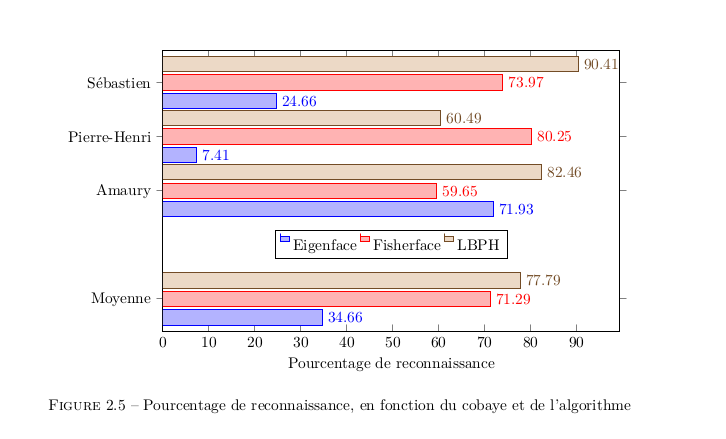
\includegraphics[scale=0.33]{images/robustesse}
			\end{center}
		\end{figure}
	\end{frame}
	\begin{frame}
		\frametitle{Description de l'algorithme LBPH}
		\begin{figure}
			\begin{center}
				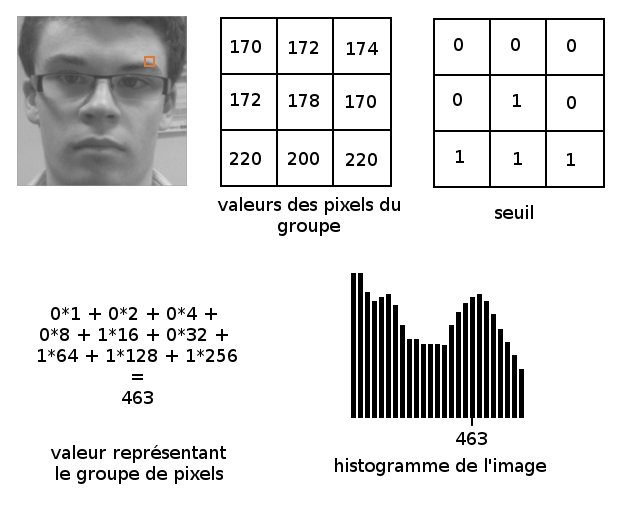
\includegraphics[scale=0.33]{images/LBPHAlgo}
			\end{center}
		\end{figure}
	\end{frame}
	\begin{frame}
		\frametitle{Pourquoi ce choix d'impl\'ementation}
		\begin{itemize}
			\item{Rapide}
			\item{Robuste}
			\item{Bien document\'e}
		\end{itemize}
		\begin{figure}
			\begin{center}
				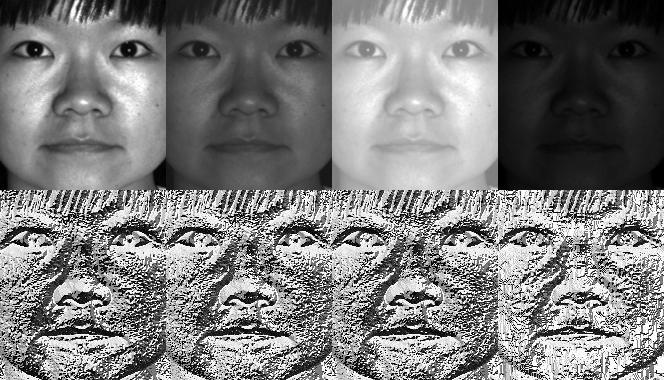
\includegraphics[scale=0.3]{images/lbphlumi}
			\end{center}
		\end{figure}
		\vfill\vfill
	\end{frame}
	\begin{frame}
		\frametitle{Probl\`emes d\'et\'ect\'es}
		\begin{itemize}
			\item{Probl\`emes au changement de luminosit\'e}
			\item{Le classifier ne d\'etecte pas que la t\^ete}
			\item{Pas impl\'ement\'ee sur la BeagleBone et la Raspberry pi}
		\end{itemize}
	\end{frame}	
	\section{Reconnaissance des \'emotions}
	\subsection{Expressions faciales}
	\begin{frame}
		\frametitle{Les 6 \'emotions primaires}
		\begin{figure}
			\begin{center}
				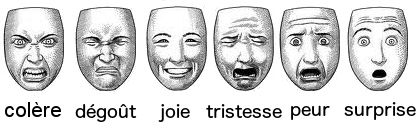
\includegraphics[scale=0.5]{images/6emotions}
			\end{center}
		\end{figure}
	\end{frame}
	\begin{frame}
		\frametitle{\'Emotions \`a d\'etecter}
		\begin{center}
			\begin{tabular}{cccc}
				
\includegraphics[height=73px]{images/tests_enerve}&
				
\includegraphics[height=73px]{images/tests_surpris}&
				
\includegraphics[height=73px]{images/tests_endormi}&
				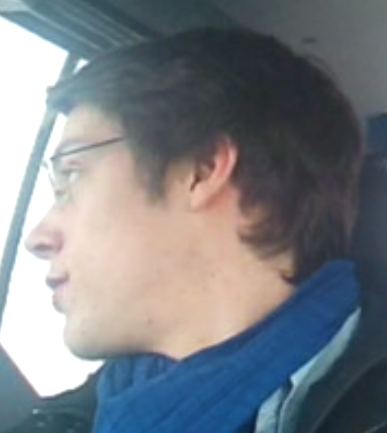
\includegraphics[height=73px]{images/tests_inattentif}\\
				\'Enerv\'e&Surpris&Endormi&Inattentif
			\end{tabular}
		\end{center}
		\vfill
	\end{frame}
	\subsection{Impl\'ementation}
	\begin{frame}
		\frametitle{Reconnaissance de la bouche}
		\begin{center}
			\begin{tabular}{c|c}
				
\includegraphics[height=30px]{images/findContoursOk}
				\hspace{5px}
				
\includegraphics[height=30px]{images/contourBouche}\hspace{5px}
				&\hspace{5px}
\includegraphics[height=30px]{images/inRangeOk}\\
				findcontour
				&couleurs
			\end{tabular}
		\end{center}
	\end{frame}
	\begin{frame}
		\frametitle{R\'esultats - Reconnaissance de la bouche}
		\begin{center}
			\begin{tabular}{cccc}
				
\includegraphics[height=65px]{images/tests_enerve}&
				
\includegraphics[height=65px]{images/tests_surpris}&
				
\includegraphics[height=65px]{images/tests_endormi}&
				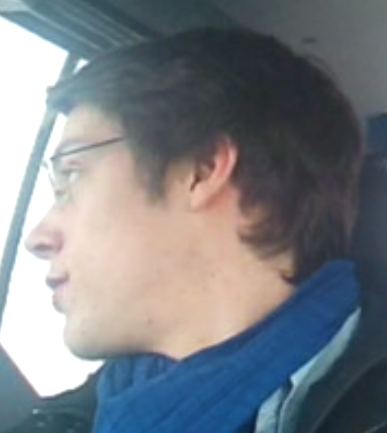
\includegraphics[height=65px]{images/tests_inattentif}\\
				\'Enerv\'e&Surpris&Endormi&Inattentif\\
				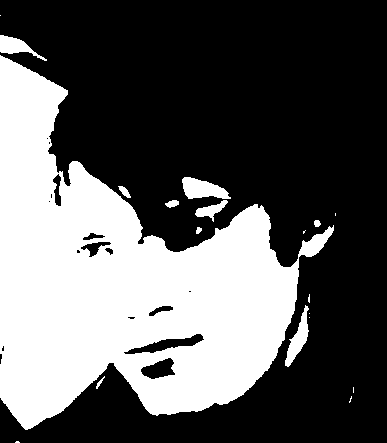
\includegraphics[height=65px]{images/finnb3}&
				
\includegraphics[height=65px]{images/finnb}&
				
\includegraphics[height=65px]{images/finnb4}&
				
\includegraphics[height=65px]{images/finnb2}
			\end{tabular}
		\end{center}
	\end{frame}
	
	\begin{frame}
		\frametitle{Reconnaissance des yeux}
		\begin{center}
			\begin{tabular}{c|c}
				
\includegraphics[height=40px]{images/findContoursYeux}\hspace{25px}
				&\hspace{25px}
\includegraphics[height=40px]{images/EyeColor}\\
				findContour
				&Couleurs
			\end{tabular}
		\end{center}
	\end{frame}
	\begin{frame}
		\frametitle{R\'esultats - Reconnaissance des yeux}
		\begin{center}
			\begin{tabular}{cccc}
				
\includegraphics[height=65px]{images/tests_enerve}&
				
\includegraphics[height=65px]{images/tests_surpris}&
				
\includegraphics[height=65px]{images/tests_endormi}&
				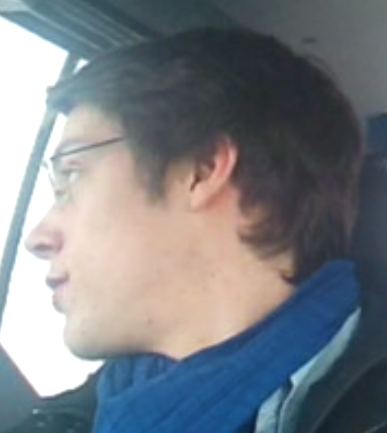
\includegraphics[height=65px]{images/tests_inattentif}\\
				\'Enerv\'e&Surpris&Endormi&Inattentif\\
				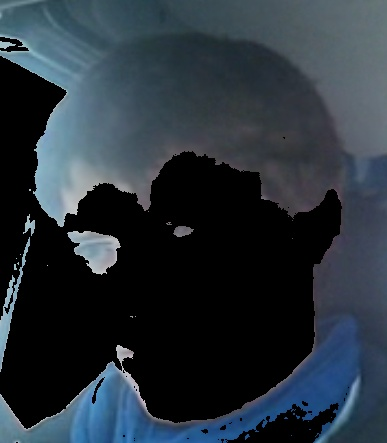
\includegraphics[height=65px]{images/fincolor2}&
				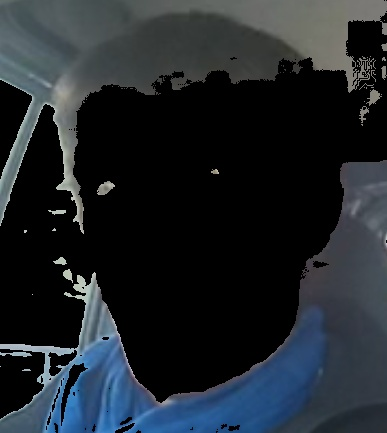
\includegraphics[height=65px]{images/fincolor}&
				
\includegraphics[height=65px]{images/fincolorendormi}&
				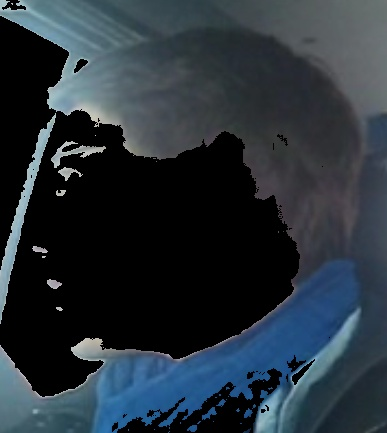
\includegraphics[height=65px]{images/fincolorin}
			\end{tabular}
		\end{center}
	\end{frame}
	
	\section{D\'emonstration}
	\subsection{tests}
	\begin{frame}
		\frametitle{Prototype de test}
		\begin{center}
			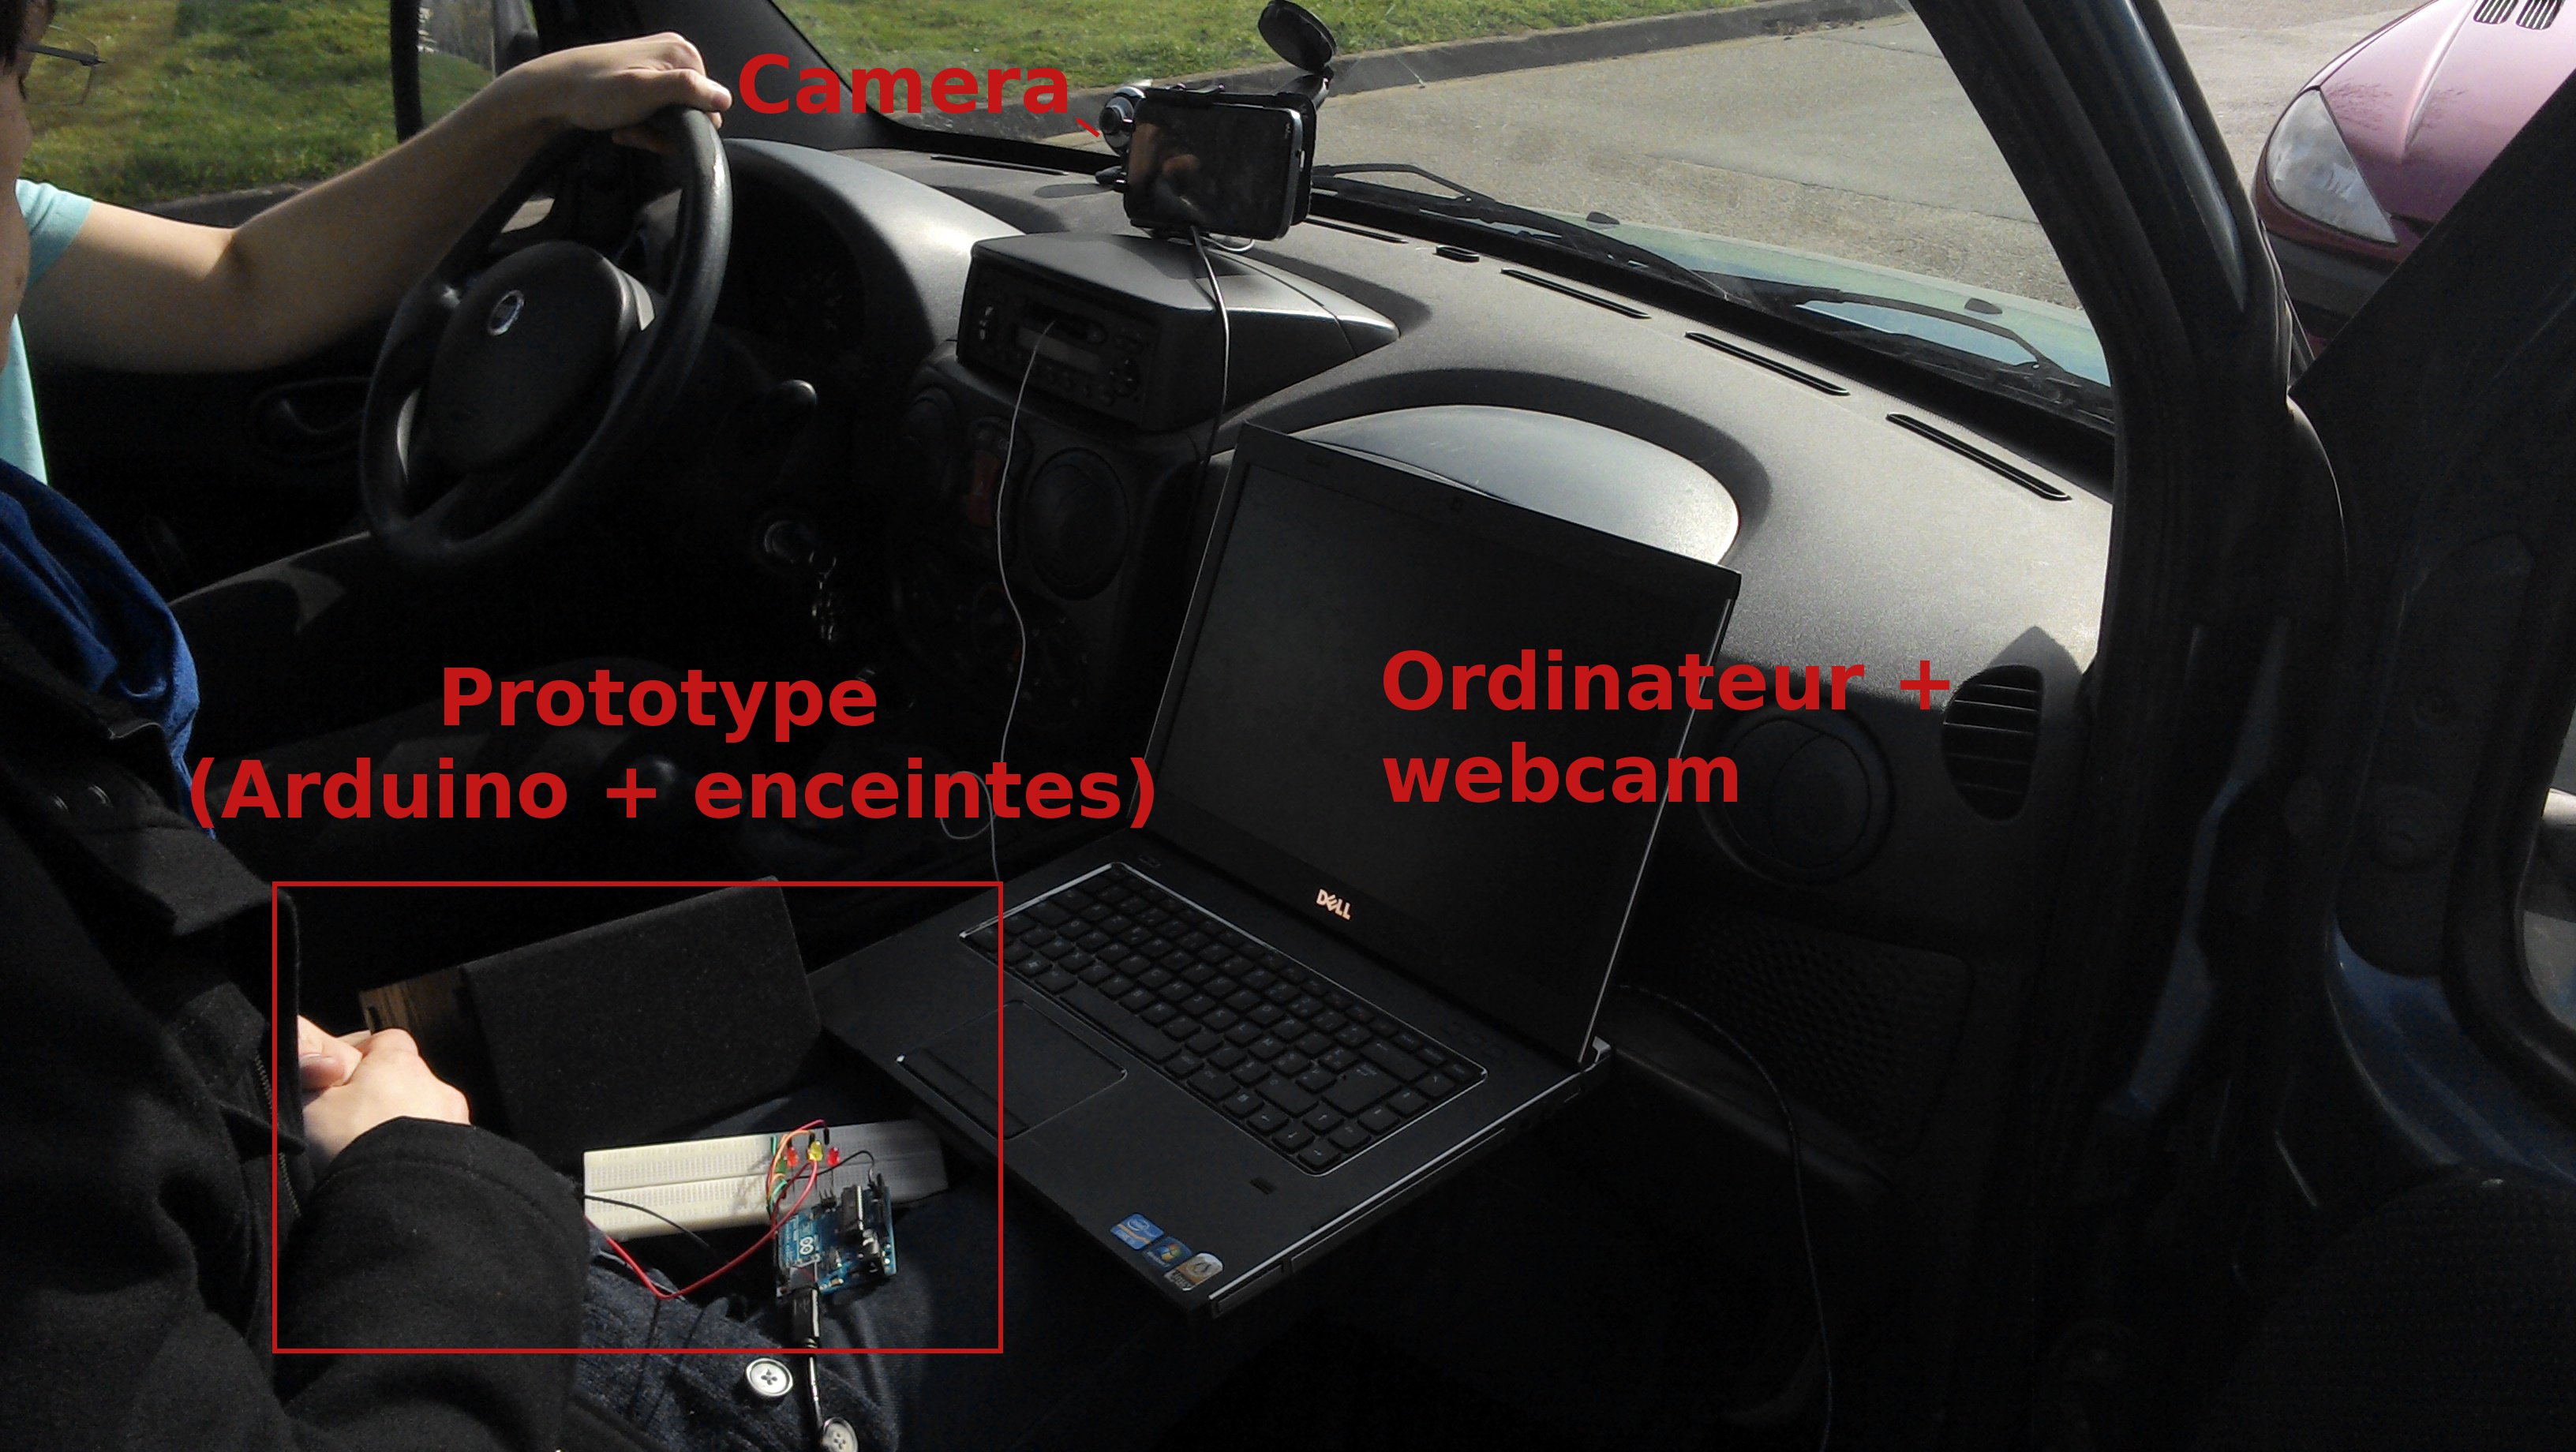
\includegraphics[scale=0.09]{images/prototype}
		\end{center}
		\hfill
	\end{frame}
	\subsection{video}
	\begin{frame}
		\frametitle{Initialisation}
		\begin{center}
			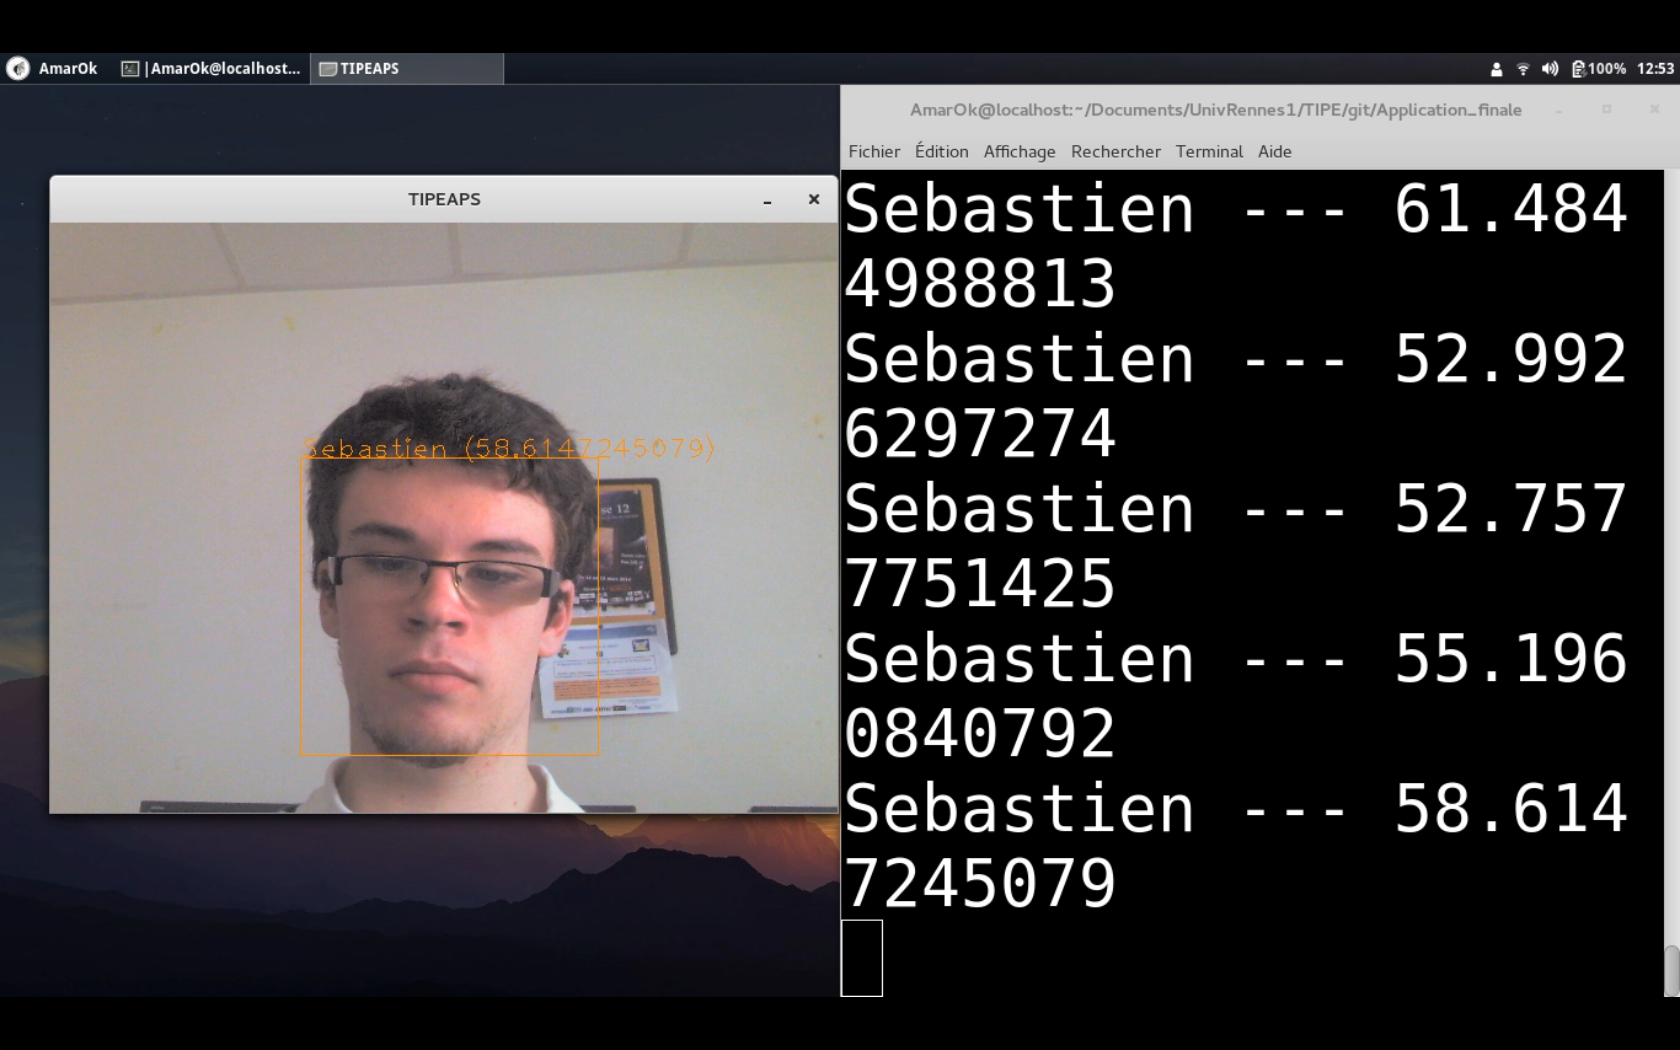
\includegraphics[scale=0.15]{images/video_init}
		\end{center}
	\end{frame}
	\begin{frame}
		\frametitle{Inattentif}
		\begin{center}
			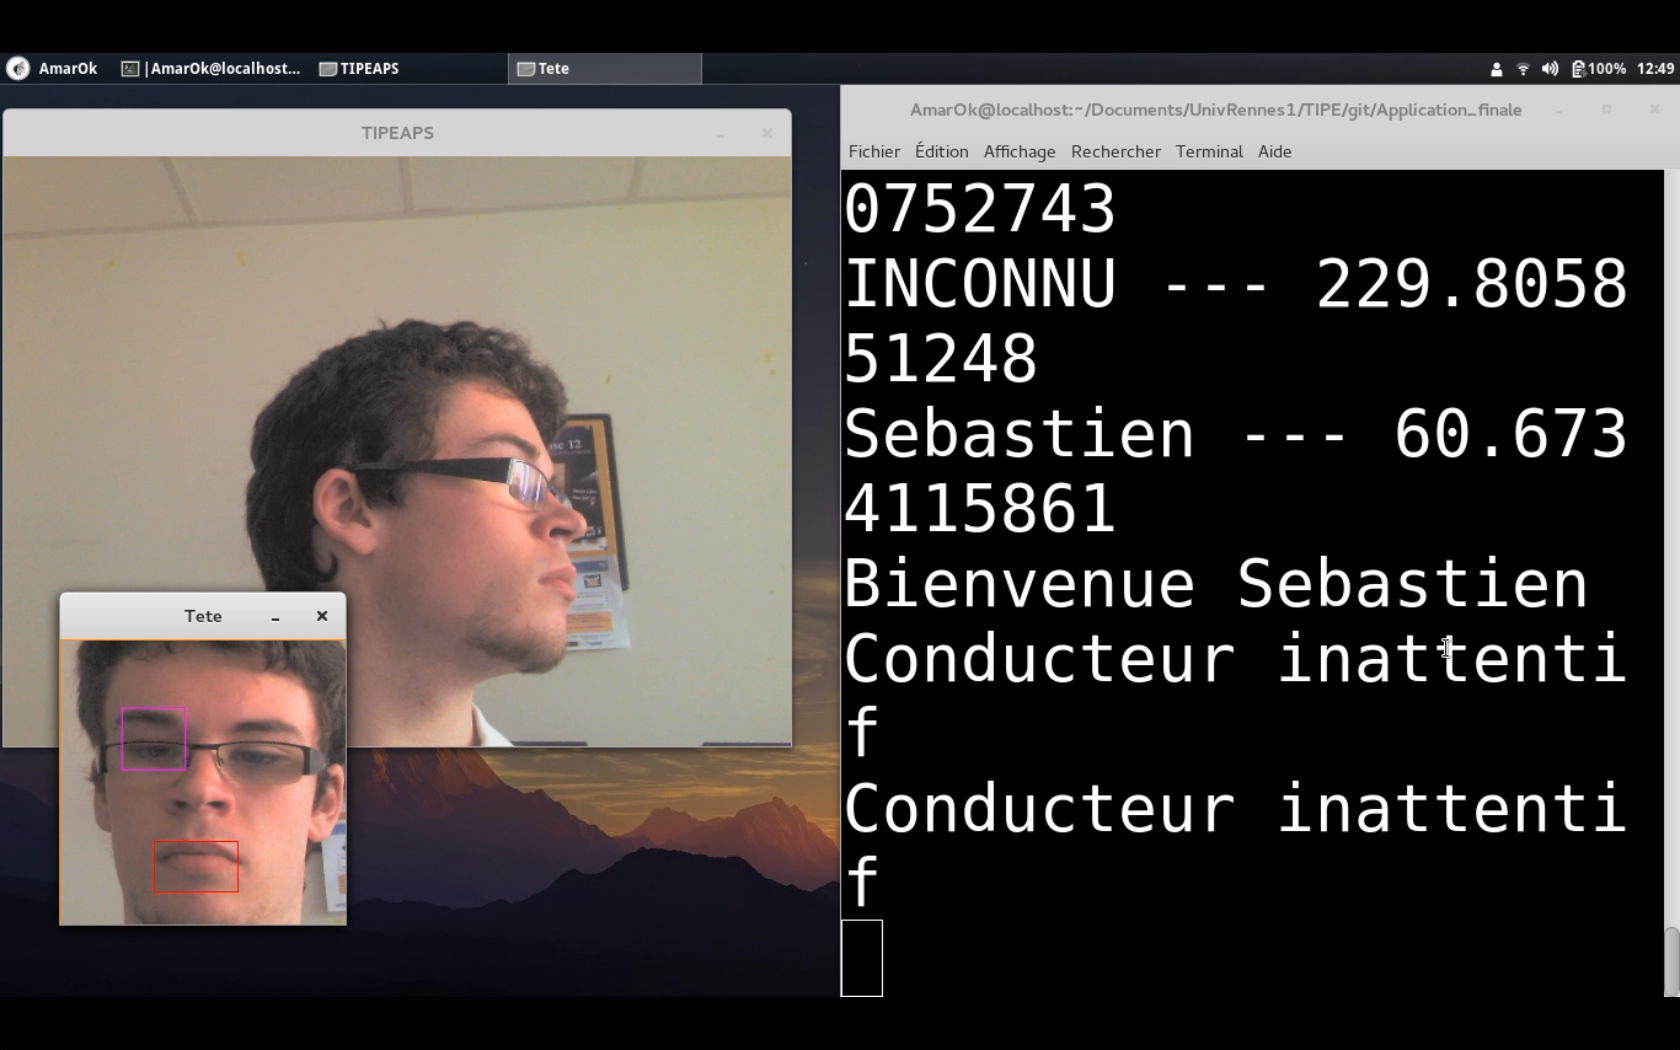
\includegraphics[scale=0.15]{images/video_inattentif}
		\end{center}
	\end{frame}
	\begin{frame}
		\frametitle{Surprise}
		\begin{center}
			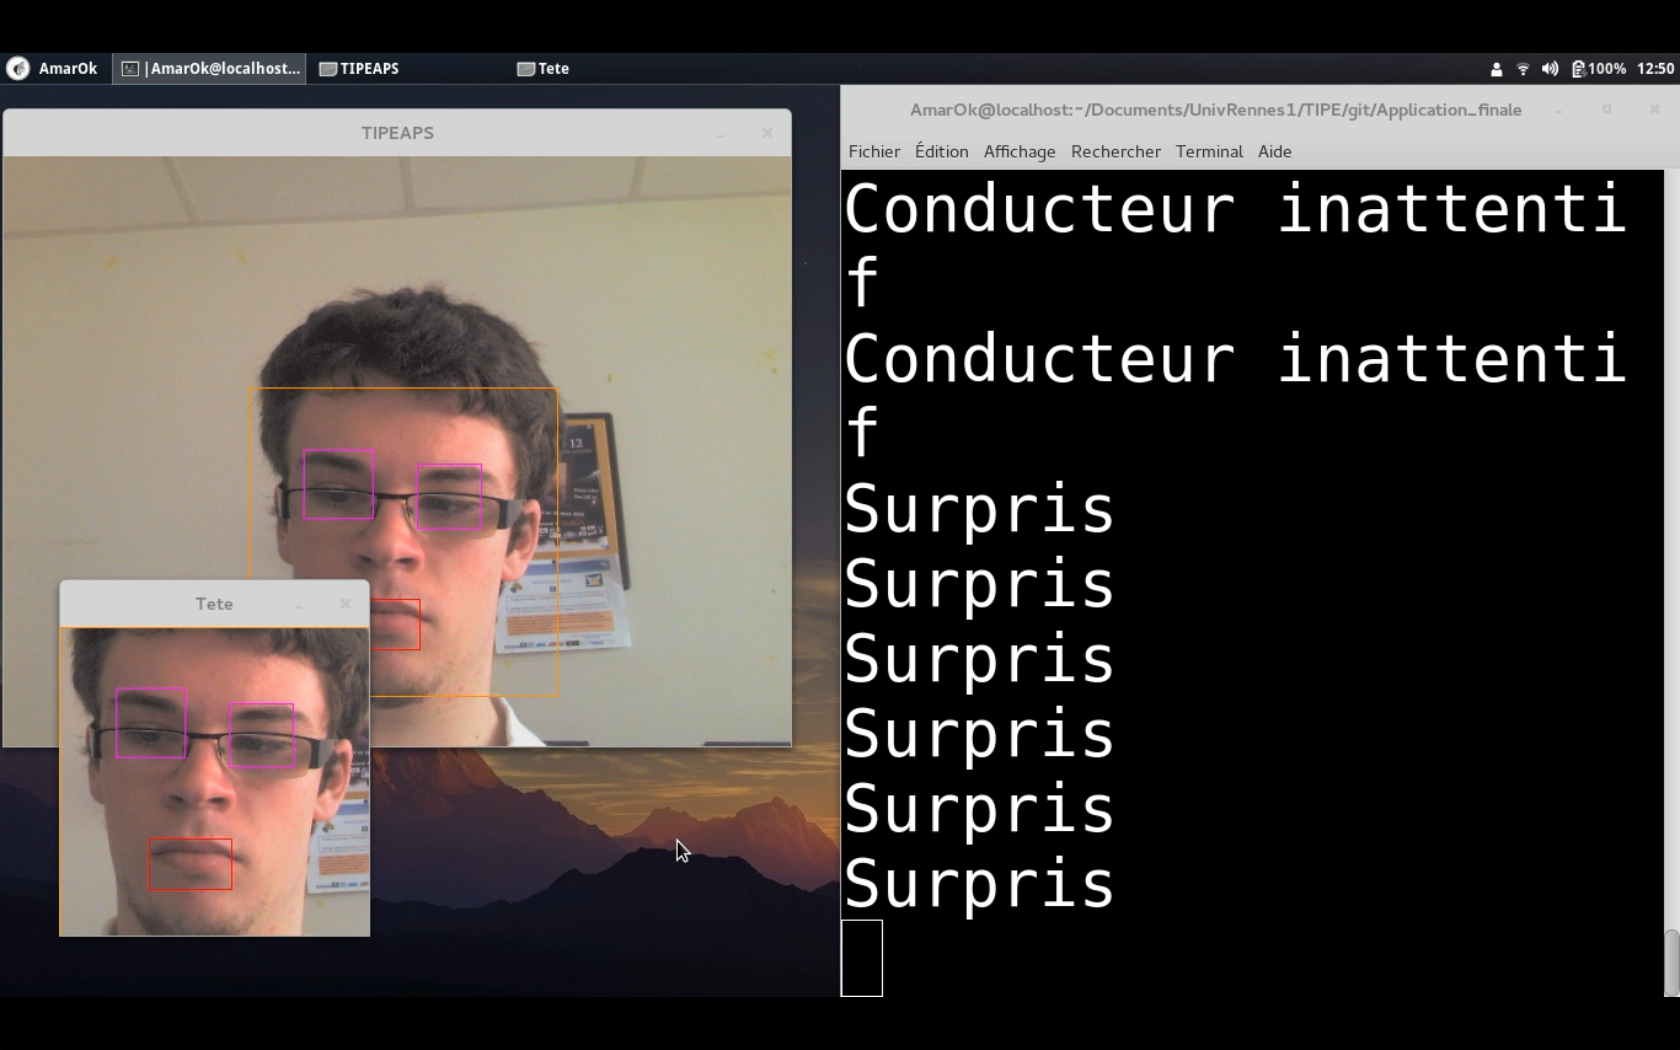
\includegraphics[scale=0.15]{images/video_surpris}
		\end{center}
	\end{frame}
	\begin{frame}
		\frametitle{\'Enervement}
		\begin{center}
			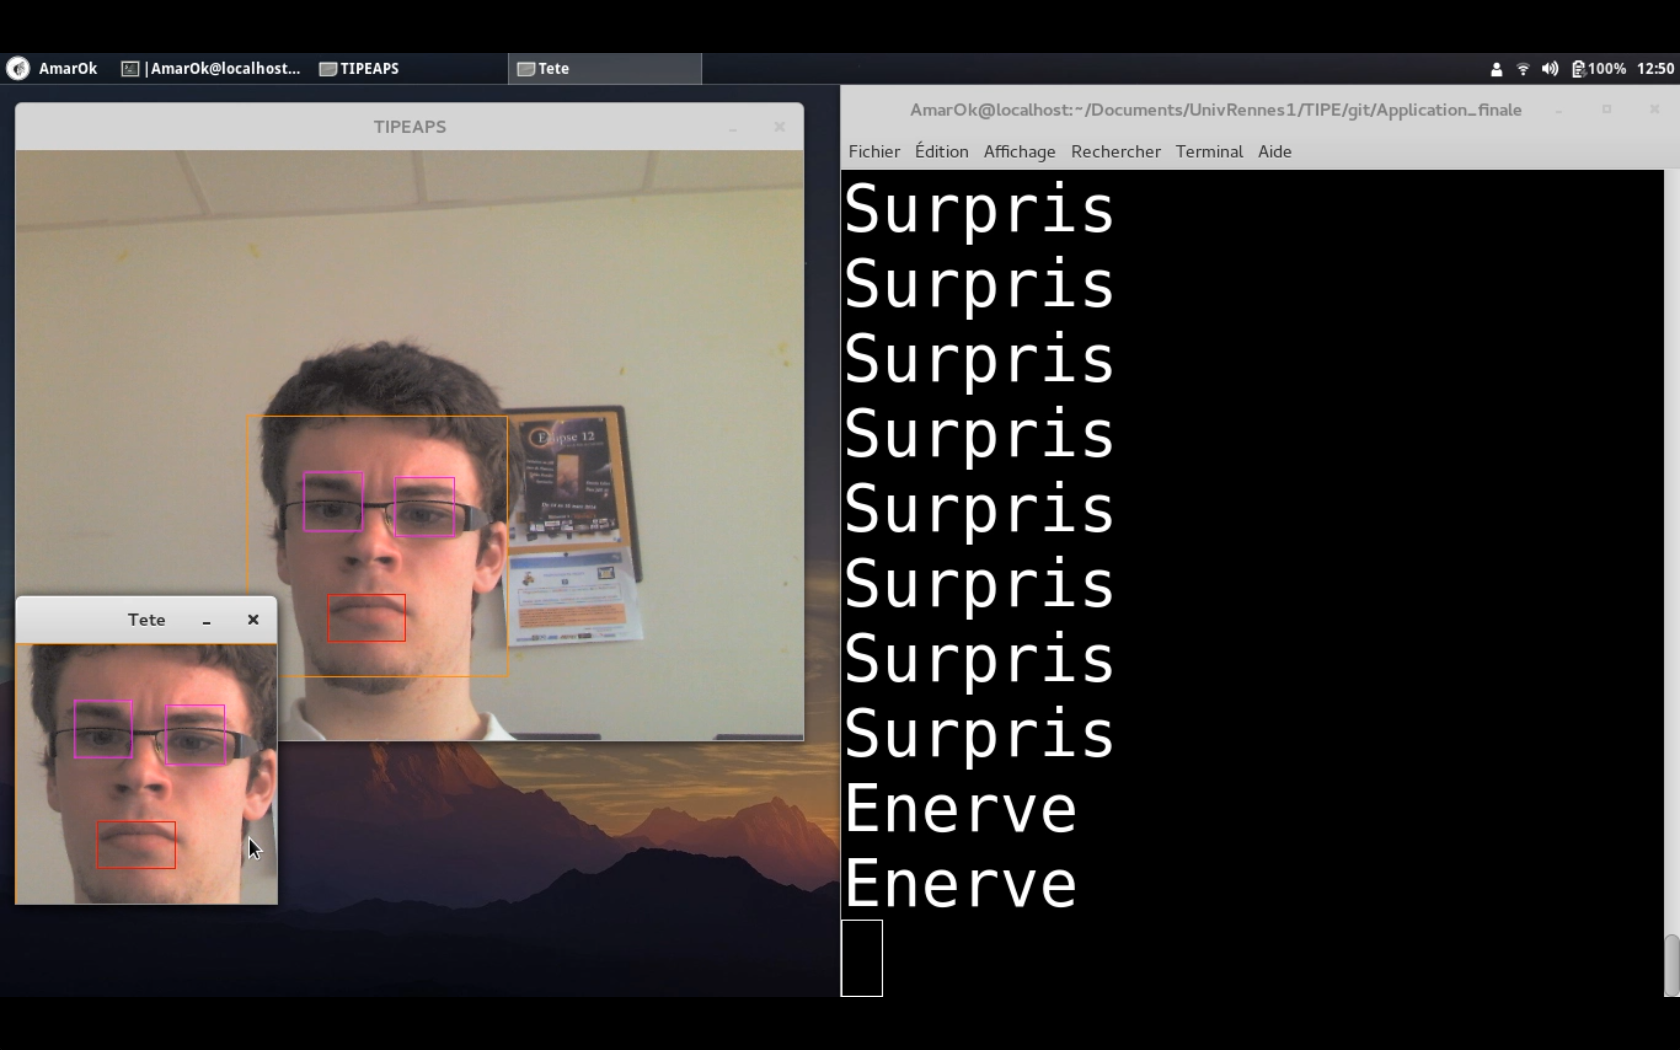
\includegraphics[scale=0.15]{images/video_enerve}
		\end{center}
	\end{frame}
	\begin{frame}
		\frametitle{Endormissement}
		\begin{center}
			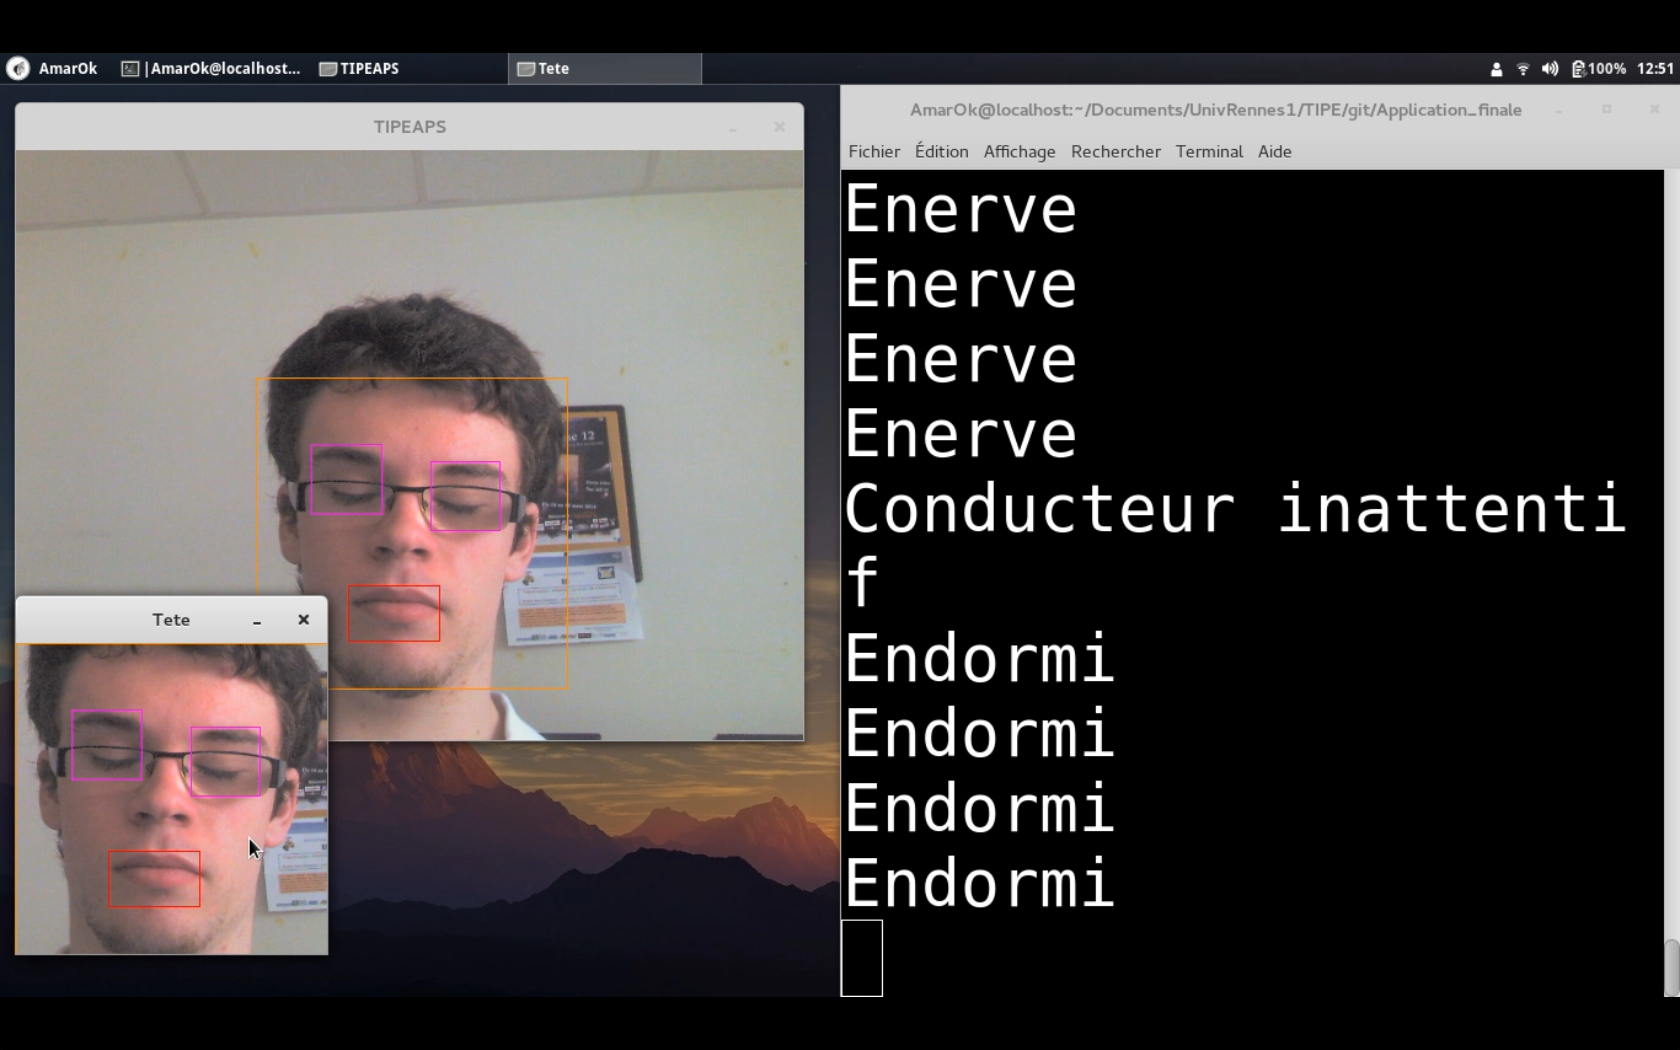
\includegraphics[scale=0.15]{images/video_endormi}
		\end{center}
	\end{frame}
	
	\section*{Conclusion}
	\subsection{Conclusion}
	\begin{frame}
		\begin{itemize}
			\item{LBPH pour la reconnaissance faciale}
			\item{D\'etection efficace de l'endormissement et de l'inattention}
			\item{D\'etection plus lente de l'\'enervement et de la surprise}
		\end{itemize}
	\end{frame}
	\begin{frame}
		\begin{block}{}
			\begin{center}
				Des questions?
			\end{center}
		\end{block}
	\end{frame}
\end{document}
	